\documentclass[a4paper,UKenglish,cleveref, autoref, thm-restate]{template/lipics-v2021}

\usepackage{float}
\usepackage{adjustbox}
\usepackage{pgfplots}

\title{AFP Project: Implementing an efficient version of Data.Map in Agda}
\author{Sebastiaan Koppen}{Utrecht University, Netherlands}{}{}{}
\author{Myrthe Streep}{Utrecht University, Netherlands}{}{}{}
\author{Daan van Westerlaak}{Utrecht University, Netherlands}{}{}{}

\authorrunning{M.D. Streep, S. Koppen, D. van Westerlaak}

\date{April 2025}

\bibliographystyle{acm}

\lstset{
  escapeinside={(*}{*)},
}

\begin{document}

\maketitle

\section{Introduction}
Data.Map is a widely used Haskell module from the containers package. It provides an optimised implementation of a dictionary-like data structure (i.e. a mapping from keys to values), based on the concept of binary search trees of bounded balance. In our initial project proposal, we suggested that such a data structure would be a useful addition to Agda. Our reasoning was that a \textit{high-quality} package would be a useful addition to Agda, as it could provide other users with a reliable, fast implementation. While we still believe in the usefulness of this implementation, we have come to learn that our initial reasoning was based on incomplete knowledge of Agda. More specifically, we now understand that speed is not a focus point of Agda, partly because it does not have a run-time in the way most languages do. Fortunately, this does not mean that our implementation is useless. A correct-by-design implementation of Data.Map can function as a tool to prove properties over Data.Map and - by extension - as a tool for identifying vulnerabilities in the data structure.

The rest of this report is layed out as follows. We will first discuss our implementation of Data.Map, as well as the sized variant and sized-balanced variant we made. We then discuss what obstacles we encountered during the project as well as some noticable things we learned. Finally we will discuss some vulnerabilities we identified in the Haskell-implementation.


\section{Implementation}
\subsection{Na\"ive implementation}
An initial implementation, based on its Haskell equivalent, can be found at \texttt{src/Map} directory. Tests and proofs corresponding to each module can be found at \texttt{src/Map/Test}. A second implementation, where the size of the map is incorporated in its type, can be found at \texttt{src/SizedMap}. Finally, an implementation incorporating both the size anf a proof of balance, can be found at \texttt{src/BalancedMap}.

When working with binary search trees, a compromise must be made between time it takes to find an element - which depends on how well-balanced the tree is - and the frequency with which the tree is rebalanced. What makes binary trees of bounded balance unique is that they carry a parameter that controls when a rebalancing is triggered. A first implementation of this can be found in the file \texttt{Map.Balance.agda}, where the constants \texttt{delta} and \texttt{ratio} are introduced. The usage of these constants corresponds to the description given by Stephen Adams \cite{adams1993functional} (although it must be pointed out that the creators of the Haskell implementation point out a small error in this paper). The \texttt{Map.Balance} module contains several functions that restore the balance of some (partially) tree. Some functions, such as \texttt{balanceL} and \texttt{balanceR}, assume that one of the sub-trees of the input is already balanced, allowing for faster rebalancing.

% We would be interested in varying these constants as part of our performance testing, as the optimal values found by the creators of Data.Map do not seem to coincide with those found by the authors of the corresponding paper.

\subsection{Sized implementation (module \texttt{SizedMap})}
The sized implementation of Data.Map incorporates the size of the map into the type (see Listing \ref{lst:sized}). The implementation of this data type was similar to the non-sized version in most situations, but in some instances the size made implementing functions more difficult. Functions like \texttt{insert} can generate a new map with an increased size as well as an equivalent size, depending on whether the inserted key was already present in the map (functions like \texttt{update} can even delete an element as well). To accomodate this, additional data types were introduced that allowed multiple types of maps (see module \texttt{SizedMap.Map}). To implement functions like \texttt{filter}, where the size of the returned map is even less predictable, the $\Sigma$ type was used to allow for a variable size.

\begin{lstlisting}[label=lst:sized,caption=Sized map. The size of a tip is zero. The size of a node is one plus the sum of the sizes of its children.]
  data Map (K : Set) (A : Set) : Nat (*$\to$*) Set where
    tip : Map K A zero
    node : K (*$\to$*) A
          (*$\to$*) Map K A m
          (*$\to$*) Map K A n
          (*$\to$*) Map K A (suc (m + n))
\end{lstlisting}

\subsection{Balanced implementation}
A third implementation of Data.Map extends the sized version with a proof of balance. This data type incorporates balance, as defined in the original Haskel implementation, into the \texttt{node} constructor (see Listing \ref{lst:balanced}).

\begin{lstlisting}[label=lst:balanced,caption=Balanced map. The size of the map is defined like in the sized implementation. An extra argument is added to the node constructor that enforces balance.]
  data BalancedMap (K : Set) (A : Set) : Nat (*$\to$*) Set where
  tip : BalancedMap K A zero
  node : K (*$\to$*) A
        (*$\to$*) (BalancedMap K A m)
        (*$\to$*) (BalancedMap K A n)
        (*$\to$*) {((m + n) (*$\le$*) 1) (*$\vee$*) ((m (*$\le$*) ((*$\delta$*) * n)) (*$\wedge$*) (n (*$\le$*) ((*$\delta$*) * m)))}
        (*$\to$*) BalancedMap K A (suc (m + n))
\end{lstlisting}


\subsection{Agda as proof assistant}
Agda was also used as proof assistant for the implemented functions, the implementations are inspired by the examples and equalities of the Hackage page of \href{https://hackage.haskell.org/package/containers-0.8/docs/Data-Map-Lazy.html}{Data.Map.Lazy}. 
Some functions are supposed to work on all instances of its record of Map.Map.agda, so to be able to formalise some proof we made an instance for it and proved that function for that instance. An example of this can be found in the function traverseWithKey of Map.Traversal with the test in Test.Traversal and the instance in Map.Map.
The proofs mostly use what was taught in the Agda lectures, but the there in $\in$ was changed to thereL and thereR to prove the branch of the element.
When some functions were proved, it became clear that there are missing cases that only arise when the function is not used properly. An example of this can be found in a part of the balanceL function in Listing \ref{balanceL}.

\begin{lstlisting}[label=balanceL,caption=balanceL assumes that the size of a node is 3 when the right branch is a tip.]
balanceL k v (node _ lk lv tip (node _ lrk lrv _ _)) tip = 
    node 3 lrk lrv (node 1 lk lv tip tip) (node 1 k v tip tip)
\end{lstlisting}

An example of a function that is proved formally is foldr which is partly shown in Listing \ref{foldrProof}. We did not expect this proof to be so hard as the function is so similar to the foldr function on lists, but the recursive calls to foldr made it harder (the elems function also uses foldr).

\begin{lstlisting}[label=foldrProof,caption=The following equality is proved foldr f z $\equiv$ foldr f z . elems]    
foldr(*$\equiv$*)foldrList-elems : {{Comparable K}} (*$\to$*) (f : A (*$\to$*) V (*$\to$*) V) 
  (*$\to$*) (z : V) (*$\to$*) (m : Map K A) (*$\to$*) foldr f z m (*$\equiv$*) foldrList f z (elems m)
foldr(*$\equiv$*)foldrList-elems f z tip = refl
foldr(*$\equiv$*)foldrList-elems f z (node x k v l r) (*$\equiv$*) 
  foldr f z (node x k v l r) 
      (*$\equiv\langle$*) ((foldr(*$\equiv$*)foldrList-elems f z r) under (f v)) 
      under ((*$\lambda$*) y (*$\to$*) foldr f y l) (*$\rangle$*)
  (foldr f (f v (foldrList f z (elems r))) l 
      (*$\equiv\langle$*) foldr(*$\equiv$*)foldrList-elems f (f v (foldrList f z (elems r))) l (*$\rangle$*)
  (foldrList f (f v (foldrList f z (elems r))) (elems l) 
      (*$\equiv\langle$*) sym (foldrList-split f z (elems l) (v :: elems r)) (*$\rangle$*)
  (foldrList f z (elems l ++ (v :: elems r)) 
      (*$\equiv\langle$*) (sym (elems(*$\equiv$*)elems  x k v l r)) under (foldrList f z) (*$\rangle$*)
  (foldrList f z (elems (node x k v l r)) (*$\blacksquare$*))))) 
\end{lstlisting}

\section{Obstacles}
Agda is very different from Haskell, both in its usage and its purpose. Using Agda for the first time proved to be quite challenging, as it requires a different way of thinking about code. At the same time, being forced into this different way of thinking also proved to be a great way to learn about concepts from lambda calculus from a more practical perspective. We will use this section to outline some of the obstacles we encountered while learning how to use Agda, as well as some of the insights it gave us. Finally, we will briefly discuss how we would approach this project if we were able to start it with the knowledge we now have.

As is to be expected when learning a new language, our first lines of code largely consisted of 'solutions' to situations where Agda's syntax was different from that of Haskell. We chose to convert the full set of Haskell modules to Agda, before moving on to benchmarking/ proofs, which on one side was a good way of learning about Agda's syntax, but on the other side resulted in perhaps a bit more code than necesary (over 1000 lines including file headers). During this process, we encountered Agda's theorem-proving properties for the first time. Functions that can fail (\texttt{find}, \texttt{findMin}, ...) are not allowed in Agda. Our approach to this was to simply exclude these functions from our implementation.

When the implementation was finished, we moved on to benchmarking and testing. Our first approach was to write single-input proofs, checking that calling some function on a specific input was equivalent to the expected result. We also attempted to write some full-coverage proofs, checking that performing a fold over a map is equivalent to performing a fold over an equivalent list. Around this time we started to realise the power that these proofs could have, as well as how complex they can get. We attempted to write a proof that inserting an element into a map results in that element being in the map. This ended up being rediculously complex and large, as our code was not written in the cleanest way and our proving skills were very limited. Plus, insert calls balance, balanceL, balanceR and several other insertion functions depending on its input. A fun, but slightly disappointing result was our discovery of some vulnerabilities in the Haskell implementation. These vulnerabilities were present because the (internal) functions make certain assumptions about the input (e.g. balanceL assumed the right sub-tree is already balanced). As a result, we were unable to finish the proof entirely.

\subsection{If we could start over..}
As mentioned several times, the learning curve for this project was steep. If we were able to start the project with our current knowledge, we would approach it in a very different way. Instead of focussing on the entire Haskell implementation, we would look at the balancing components - including functions like insert that use the balancing components - and attempt to write a correct-by-construction implementation. We would incorporate balancing and size properties into the data type and attempt to write a simplified implementation where the tree would be rebalanced based on those properties. While we started doing this in the \texttt{BalancedMap} directory, we spent only a small portion of the available time on it. The result would be an implementation that could be translated to Haskell (or other languages), providing a proven-correct implementation in a (efficient) production language. While this translation would entail removing the balancing and size properties from the data structure, the Agda-progam would still provide a proof of correctness. In other words, we should have done the project the other way around.


\section{Performance}
% At the start of this project, none of the group members had any experience with Agda or other interactive theorem provers. Because of this, the (faulty) assumption was made that Agda is a language that can be used for production code. While the tool MAlonzo can be used to compile Agda code to Haskell, the resulting code is - in our experience - not optimised for performance and cannot be compared to code written directly in Haskell. As a result, our original plan of comparing the Agda implementation to the original Haskell implementation turned out to be fun, but not very interesting from a 'results' perspective.


Not long after we started implementing code in Agda, we realized Agda was different from many languages in a way that we had not anticipated. This difference, namely the the fact that Agda did not seem to compile in the traditional sense, had us realize that benchmarking too would not work the way we traditionally would.\newline

We had heard that it was possible to transpile Agda code to Haskell, so this seemed to be a logical step to take in order to benchmark our Agda against Haskell. However, this would mean we would in actuality be comparing generated Haskell against normal Haskell, which sounded less meaningful than benchmarking Agda directly. As such, we decided to ask about benchmarking Agda in the next meeting we would have with Lawrence.
 
Here we were adviced to try and benchmark Agda as ran from the command line. If we would make sure to delete cache files, this would allow us to time the duration of the resolver for Agda. While this would not get us any data that could meaningfully be compared to Haskell, it would be data that is most closely related to Agda.\newline

Out of curiosity we also still wanted to benchmark the transpiled Agda code against Haskell. For timing Agda from the command line, we were recommended the hyperfine tool, and as such we decided to check it out. We found that hyperfine had support for timing multiple commands in batch, as well as having support for exporting the results. The tool looked promising and as such we prepared a script and started to benchmark our Agda code.\newline

While we were not sure what kind of data to expect, running the script nevertheless proved disappointing. This was not because of the data we got, but rather the data we didn't get; hyperfine reported an error. It appeared hyperfine was unable to find Agda, so we confirmed it should be able to find Agda, and subsequently hardcoded the path to Agda so that absolutely should be found. We ran the script again, once more being told that Agda could not be found.\newline

While it seemed illogical, we figured that something about the script might be the issue, and ran hyperfine from the command line manually. It once again reported that Agda could not be found, yet we were able to run Agda manually from the exact same command prompt. We experimented further and found that hyperfine appeared to report the same error for any input we gave it, and as such we concluded that hyperfine itself was not working correctly. Neither reinstalling, nor building from source was able to get hyperfine to work.
 
 -- TODO: cite hyperfine ?
 
For the comparison between the Agda transpiled to Haskell and normal Haskell, we used Criterion. Criterion offers a function that evaluates results to normal form, and makes sure that optimization does not cause evaluation to only happen for the first iteration in a benchmark. The benchmarking is based on the dictionaries repo of the Haskell performance Github organization.

Some of the benchmarking data can be seen in table. -- TODO: reference figure/table
Due to how Agda transpiles to Haskell, not all functions were able to adequately be benchmarked.

-- TODO: table

-- TODO: observations ?

-- TODO: cite Criterion ?
-- TODO: cite ``Haskell performance'' dictionaries repo


\begin{figure}[htbp]
  \centering
  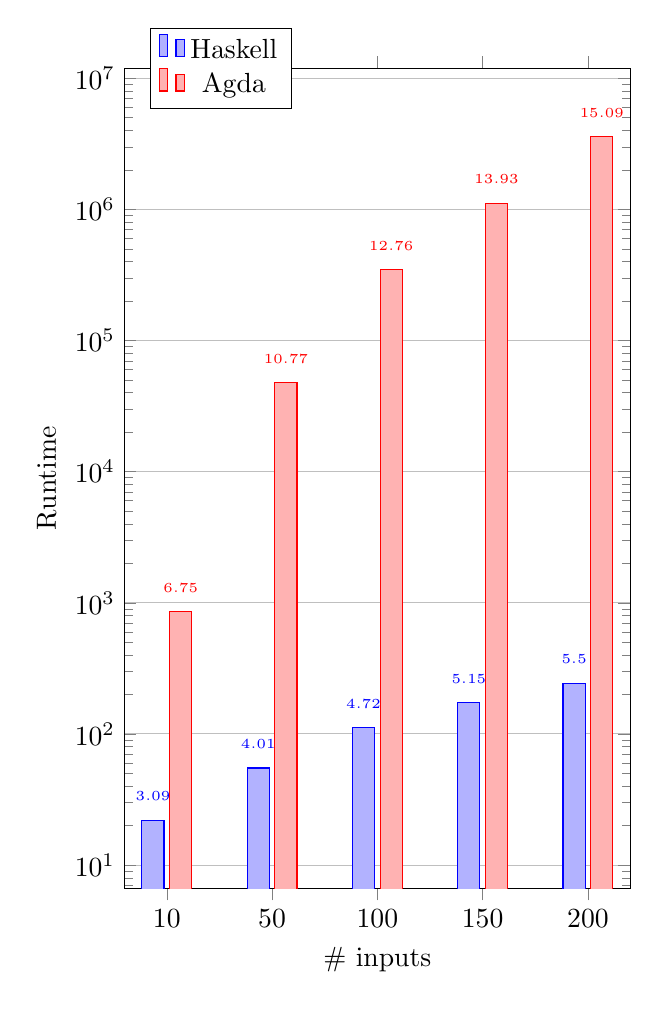
\begin{tikzpicture}
      \begin{axis}[
        ymajorgrids=true,
        ymode=log,
        ybar,
        symbolic x coords={10, 50, 100, 150, 200},
        bar width=8pt,
        enlarge x limits=0.1,
        nodes near coords,
        ylabel={Runtime},
        xlabel={\# inputs},
        xtick=data,
        ytick={1,10,100,1000,10000,100000,1000000,10000000},
        every node near coord/.append style={font=\tiny, yshift=3.5pt},
        height=12cm,
        width=8cm,
        legend style={at={(0.05,1)},anchor=west}
      ]
      \addplot coordinates {(10,22) (50, 55) (100, 112) (150, 173) (200, 244)};
      \addplot coordinates {(10,857.5) (50, 47770) (100, 346500) (150, 1117000) (200, 3593000)};
      \legend{Haskell, Agda}
      \end{axis}

  \end{tikzpicture}
  \caption{The runtime for different amounts of inputs for the insert function. As can be seen, Haskell outperforms Agda by several orders of magnitude. It also appears that Haskell has slightly worse than linear complexity, while Agda has exponential complexity.}
\end{figure}

\section{Conclusion}




\bibliography{main}
\end{document}
